En esta sección se detallan las especificaciones de los casos de uso identificados para el proyecto. 

Los casos de uso son descripciones de las interacciones entre los actores y el sistema y son fundamentales para la definición de los requisitos funcionales del mismo.

La especificación de cada caso de uso se ha basado en las recomendaciones de Cockburn \cite{cockburn2000writing}. Cada caso de uso incluye los siguientes elementos:
\begin{itemize}
    \item \textbf{Nombre del caso de uso}: un nombre corto y descriptivo.
    \item \textbf{Descripción}: una descripción general del caso de uso.
    \item \textbf{Actores principales}: los actores que inician el caso de uso.
    \item \textbf{Actores secundarios}: los actores que participan en el caso de uso, pero no lo inician.
    \item \textbf{Precondiciones}: las condiciones que deben cumplirse antes de que el caso de uso pueda comenzar.
    \item \textbf{Postcondiciones}: las condiciones que deben cumplirse al finalizar el caso de uso.
    \item \textbf{Disparadores}: los eventos que inician el caso de uso.
    \item \textbf{Escenario principal}: la secuencia de pasos que describe la interacción entre los actores y el sistema.
    \item \textbf{Escenarios alternativos}: descripciones de las ramificaciones del escenario principal.
    \item \textbf{Situaciones de error}: descripciones de las situaciones en las que el caso de uso puede fallar.
\end{itemize}
% https://www-public.imtbs-tsp.eu/~gibson/Teaching/Teaching-ReadingMaterial/Cockburn00.pdf


Los casos de uso están organizados en secciones según el actor que los inicie. Los actores han sido previamente identificados y descritos en el apartado denominado
\coloredUnderline{\hyperlink{sec:6_1-Identificacion_actores}{\ref*{sec:6_1-Identificacion_actores} \nameref*{sec:6_1-Identificacion_actores}}}.

En la figura \coloredUnderline{\hyperlink{fig:diagrama_contexto}{Figura \ref*{fig:diagrama_contexto}: \nameref*{fig:diagrama_contexto}}}
se muestra el diagrama de contexto del sistema, que representa las interacciones entre los actores y el sistema. 
Este diagrama introduce los casos de uso que se describen en las siguientes secciones.

\begin{figure}[H]
    \centering
    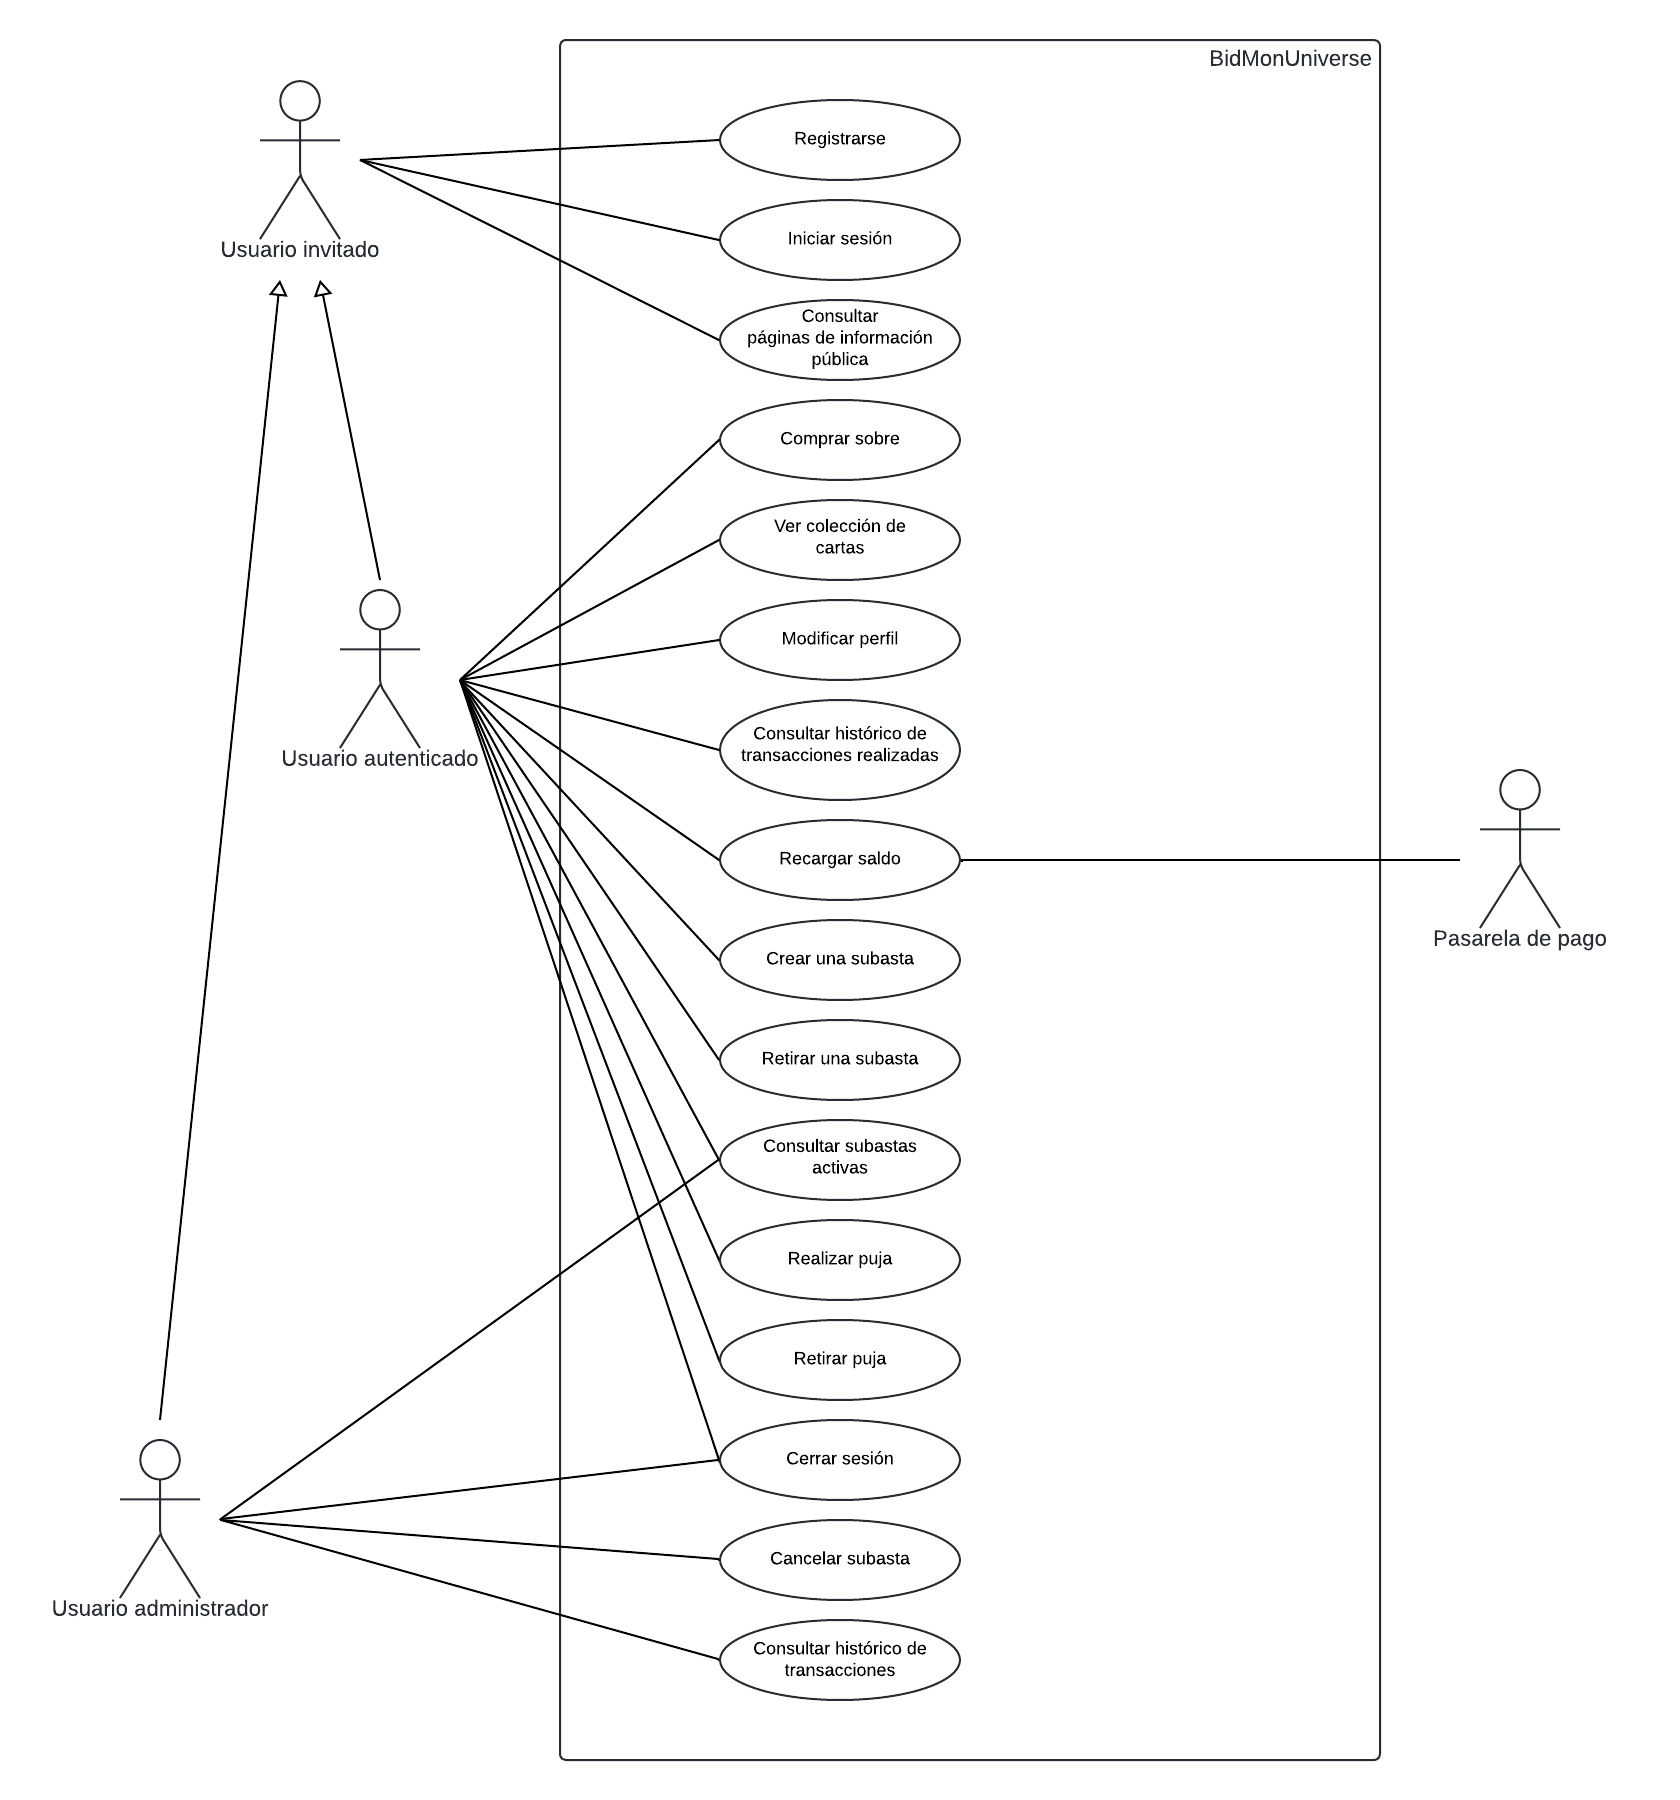
\includegraphics[width=0.9\textwidth]{figures/6-Analisis/6-Casos-uso/6_Diagrama-contexto.png}
    \caption{Diagrama de contexto del sistema}
    \label{fig:diagrama_contexto}
\end{figure}

\subsection{Casos de uso: Registro}

\begin{table}[H]
\centering
\caption{Caso de Uso: Registro}
\label{table:usecase}
\begin{tabular}{
  >{\columncolor{lightgreen!20}}p{4cm}
  p{10cm}
}
\toprule
\rowcolor{darkgreen!50}
\textbf{Nombre} & \multicolumn{1}{>{\columncolor{darkgreen!50}\centering\arraybackslash}p{10cm}}{\textbf{REGISTRO}} \\
\midrule
Descripción & Una descripción general del caso de uso \\
\midrule
Actores principales & Los actores que inician el caso de uso \\
\midrule
Actores secundarios & Los actores que participan, pero no inician el caso de uso \\
\midrule
Precondiciones & Condiciones previas necesarias para que el caso de uso comience \\
\midrule
Postcondiciones & Condiciones que se establecen una vez finalizado el caso de uso \\
\midrule
Disparadores & Eventos que dan inicio al caso de uso \\
\midrule
Escenario principal & Secuencia de pasos principal entre actores y el sistema \\
\midrule
Escenarios alternativos & Ramificaciones del escenario principal \\
\midrule
Situaciones de error & Situaciones en las que el caso de uso puede fallar \\
\bottomrule
\end{tabular}
\end{table}
